The cross spectrum magnitudes were obtained by spectral multiplication of the regular spectrum of one receiver with the complex conjugate spectrum of the other receiver and are shown in figures \ref{fig:t4-mag-2-3} to \ref{fig:t4-phase-4-5}.
Here, only two cross spectra are shown. The rest can be found in the appendix \ref{app:xspec}. Looking at the magnitude plots, one finds an increase in the signal amplitude values. So in comparison to the coherent integration method, which does not increase the amplitude values, this cross spectrum method improves SNR by just that method.\\


\begin{figure}
    \centering
    \begin{minipage}{0.48\textwidth}
        \centering
        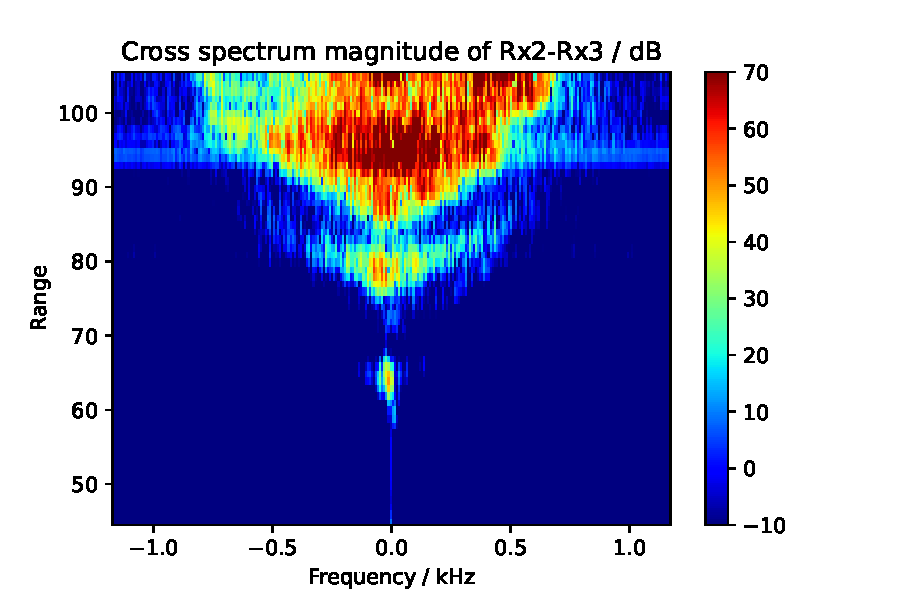
\includegraphics[width=\textwidth]{graphics/t4/t4-mag-2-3.pdf}
    \caption{Task 4: Magnitude of cross spectrum of Receivers 2 and 3.}
    \label{fig:t4-mag-2-3}
    \end{minipage}\hfill
    \begin{minipage}{0.48\textwidth}
        \centering
             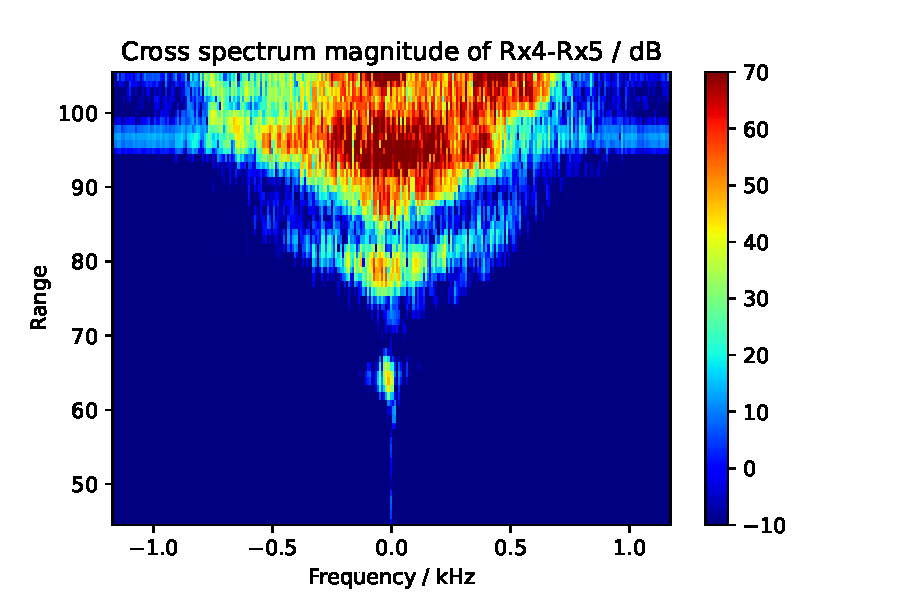
\includegraphics[width=\textwidth]{graphics/t4/t4-mag-4-5.pdf}
    \caption{Task 4: Magnitude of cross spectrum of Receivers 4 and 5.}
    \label{fig:t4-mag-4-5}
    \end{minipage}
\end{figure}

\begin{figure}
    \centering
    \begin{minipage}{0.48\textwidth}
        \centering
        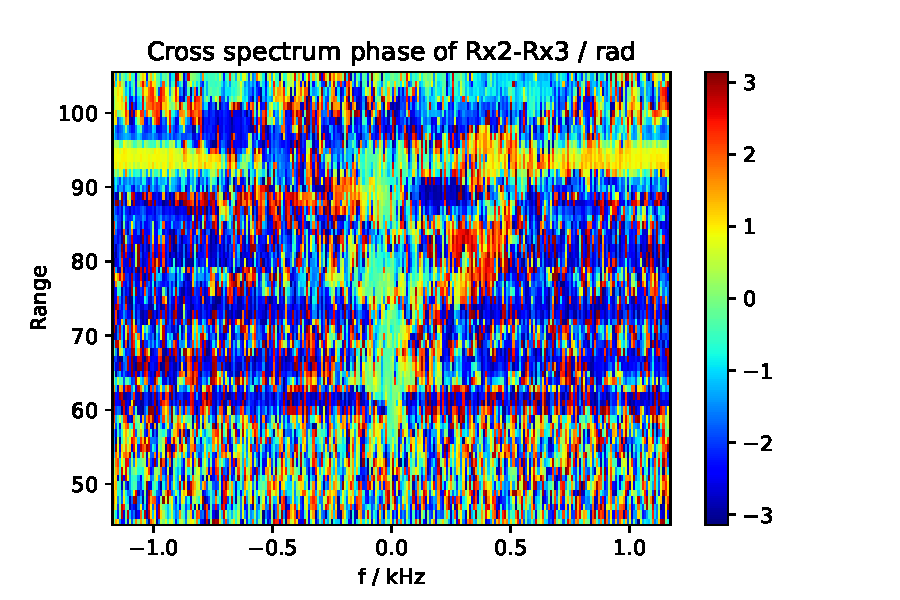
\includegraphics[width=\textwidth]{graphics/t4/t4-phase-2-3.pdf}
    \caption{Task 4: Phase of cross spectrum of Receivers 2 and 3.}
    \label{fig:t4-phase-2-3}
    \end{minipage}\hfill
    \begin{minipage}{0.48\textwidth}
        \centering
        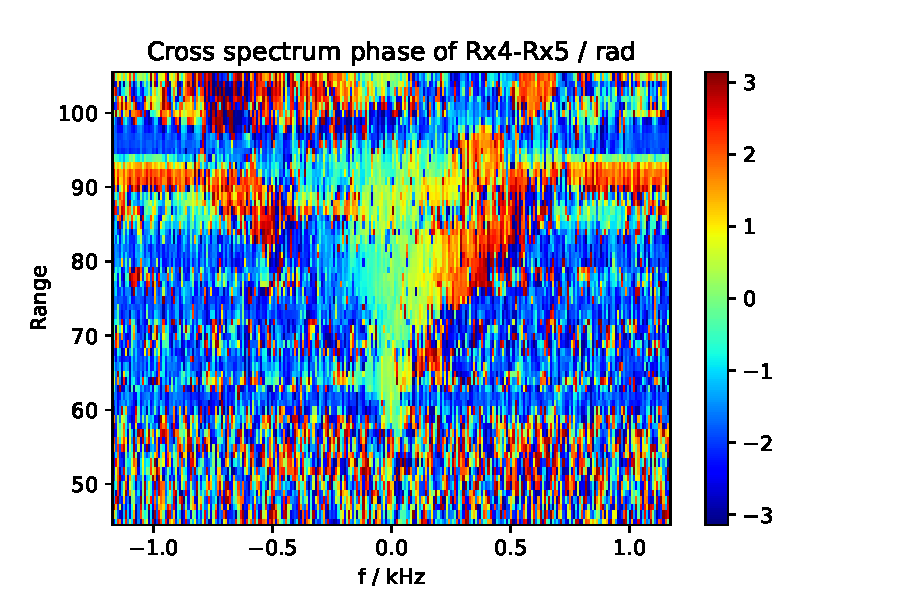
\includegraphics[width=\textwidth]{graphics/t4/t4-phase-4-5.pdf}
    \caption{Task 4: Phase of cross spectrum of Receivers 4 and 5.}
    \label{fig:t4-phase-4-5}
    \end{minipage}
\end{figure}
